%%%%%%%%%%%%%%%%%%%%%%%%%%%%%%%%%%%%%%%%%%%%%%%%%%%%%%%%%%%

\section{Apresentação dos dados}

O problema de classificação com o reconhecimento de atividades humanas utiliza como base de dados amostras tomadas do acelerômetro e do giroscópio do \textit{smartphone} preso à cintura do candidato. Dessa forma, com base na leitura desses sensores, pode-se identificar se a pessoa está caminhando, subindo escadas, descendo escadas, sentada, de pé ou deitada, que representam as seis classes do problema.

Além dos dados brutos, é fornecido também os dados processados, com extração sobre os dados no tempo, na frequência, e também características estatísticas dos mesmos.

\subsection{Dados tratados}

Os dados tratados são formados por amostras de 561 atributos derivados da análise no tempo e na frequência dos dados provenientes do acelerômetro e do giroscópio do \textit{smartphone}. São um total de 7352 amostras para treinamento e validação, e 2947 amostras para teste.

O balanceamento das classes nos conjuntos de dados foi realizado por meio do cálculo da taxa de ocorrência dos mesmos, dada de acordo com \eqref{eq:rate}. A \autoref{fig:balancingofclasses} mostra a distribuição das classes, e pode-se ver que não existe um balanceamento homogêneo, onde a classe 3 é a que menos ocorre, enquanto a classe  6 é a que mais ocorre.

Devido a esse desbalanceamento, a métrica que será utilizada para a avaliação do desempenho de cada classificador será a acurácia balanceada, dada por \eqref{eq:ba}.

\begin{equation}\label{eq:rate}
	Rate_i = \frac{N_i}{N}
\end{equation}

% TODO: \usepackage{graphicx} required
\begin{figure}[H]
	\centering
	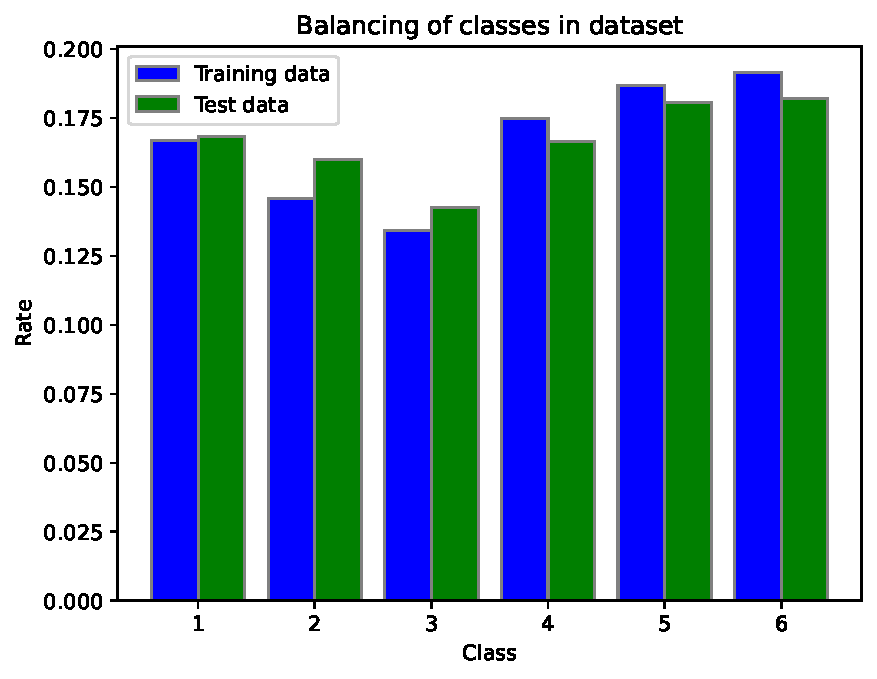
\includegraphics[width=0.75\linewidth]{../../plot/Balancing_of_classes}
	\caption{Gráfico da ocorrência das classes nos conjuntos de dados de treinamento e teste.}
	\label{fig:balancingofclasses}
\end{figure}

\begin{equation}\label{eq:ba}
	BA = \frac{\sum_{i=1}^{Q}Recall_i}{Q} = \frac{\sum_{i=1}^{Q}\frac{\text{TP}_i}{N_i}}{Q} = \frac{\sum_{i=1}^{Q}\frac{\text{TP}_i}{N\cdot Rate_i}}{Q}
\end{equation}



%%%%%%%%%%%%%%%%%%%%%%%%%%%%%%%%%%%%%%%%%%%%%%%%%%%%%%%%%%%

\section{Classificação via Regressão Logística}




%%%%%%%%%%%%%%%%%%%%%%%%%%%%%%%%%%%%%%%%%%%%%%%%%%%%%%%%%%%
\subsection{Dados tratados}

\subsubsection{Estrutura de treinamento}





\subsubsection{Passo de evolução}









%%%%%%%%%%%%%%%%%%%%%%%%%%%%%%%%%%%%%%%%%%%%%%%%%%%%%%%%%%%
\subsection{Dados brutos}







%%%%%%%%%%%%%%%%%%%%%%%%%%%%%%%%%%%%%%%%%%%%%%%%%%%%%%%%%%%

\section{Classificação via \textit{k neareast neighbours}}

A classificação pelo método \textit{k neareast neighbours} é baseada em inferir a classe do dado a ser classificado com base nos $k$ dados mais próximos à ele. Como hiper-parâmetros para esse problema, têm-se principalmente o valor de $k$, a ordem $p$ da distância de Minkowski entre os dados e o critério de classificação.

O critério de classificação pode se basear puramente na classe majoritária entre os $k$ vizinhos, ou levar em consideração a distância como um peso, que normalmente é inversamente proporcional a distância, evidenciando o rótulo dos pontos mais próximos do dado teste.


%%%%%%%%%%%%%%%%%%%%%%%%%%%%%%%%%%%%%%%%%%%%%%%%%%%%%%%%%%%
\subsection{Dados tratados}

Para implementação do algoritmo de \textit{k}NN, foi escolhido a utilização da distância euclidiana no espaço dos atributos, e a decisão do rótulo vencedor por meio do voto majoritário dos $k$ vizinhos mais próximos.

Para obtenção do valor de $k$, foi executada uma busca em \textit{grid} do hiper-parâmetro, variando seu valor entre 1 e 30. Utilizando os dados de teste, buscando suas classes por meio da inferência no conjunto de dados de treinamento, foi calculada a acurácia balanceada para cada número de vizinhos testado. A \autoref{fig:gridsearch} exibe a evolução da acurácia balanceada para os valores de $k$, e com isso, resulta-se que o valor ótimo para o classificador é $k = 8$.


% TODO: \usepackage{graphicx} required
\begin{figure}[H]
	\centering
	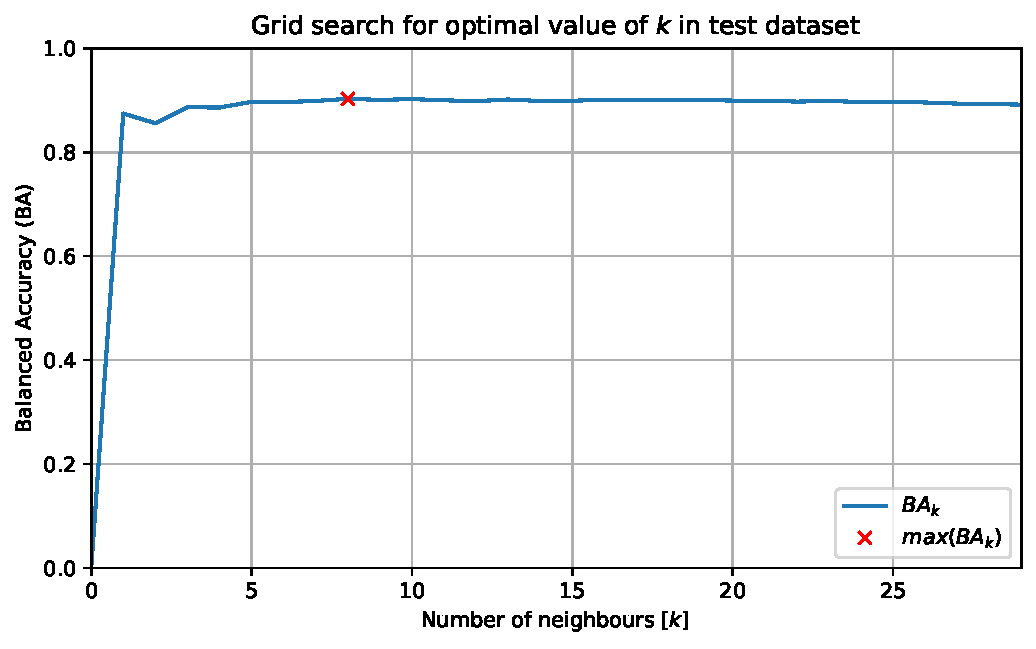
\includegraphics[width=0.75\linewidth]{../../plot/knn_1/grid_search}
	\caption{Busca em \textit{grid} do valor de $k$ ótimo.}
	\label{fig:gridsearch}
\end{figure}

Uma vez definido o classificador ótimo, obtém-se os indicadores de performance do classificador. A acurácia balanceada encontrada foi de 0,9028 e a matriz de confusão do classificador por ser vista na \autoref{tab:mc_knn_1}.

\begin{equation}\label{eq:ba_knn_1}
	BA = 0,9028
\end{equation}

\begin{table}[H]
	\centering
	\begin{tabular}{c||c|c|c|c|c|c|}
		\cline{2-7}
		& \textbf{1} & \textbf{2} & \textbf{3} & \textbf{4} & \textbf{5} & \multicolumn{1}{l|}{\textbf{6}} \\ \hline \hline
		\multicolumn{1}{|c||}{\textbf{1}} & 486        & 1          & 9          & 0          & 0          & 0                               \\ \hline
		\multicolumn{1}{|c||}{\textbf{2}} & 42         & 426        & 3          & 0          & 0          & 0                               \\ \hline
		\multicolumn{1}{|c||}{\textbf{3}} & 51         & 42         & 327        & 0          & 0          & 0                               \\ \hline
		\multicolumn{1}{|c||}{\textbf{4}} & 0          & 4          & 0          & 420        & 67         & 0                               \\ \hline
		\multicolumn{1}{|c||}{\textbf{5}} & 0          & 0          & 0          & 51         & 481        & 0                               \\ \hline
		\multicolumn{1}{|c||}{\textbf{6}} & 0          & 0          & 0          & 2          & 1          & 534                             \\ \hline
	\end{tabular}
	\caption{Matriz de confusão do classificador k-NN com k = 8.}
	\label{tab:mc_knn_1}
\end{table}

Extraindo da matriz de confusão as métricas de precisão e \textit{recall}, obtém-se a \autoref{tab:pr_knn_1}. Pode-se observar que a classe 3 foi a que apresentou menor precisão, sendo muito confundida com a classe 1 e 2. Já a classe 1 possuí o pior \textit{recall}, uma vez que as classes 2 e 3 se confundem com a 1. A classe 6 foi a que apresentou o melhor desempenho, apresentando \textit{recall} unitário, logo, nenhuma classe se confunde com ela, e a maior precisão, muito próxima de 1.


\begin{table}[H]
	\centering
	\begin{tabular}{c|c|c}
		\textbf{Classe} & \textbf{Precisão} & \textbf{\textit{Recall}} \\ \hline
		\textbf{1}      & 0,9798            & 0,8394          \\
		\textbf{2}      & 0,9045            & 0,9006          \\
		\textbf{3}      & 0,7786            & 0,9646          \\
		\textbf{4}      & 0,8554            & 0,8879          \\
		\textbf{5}      & 0,9041            & 0,8761          \\
		\textbf{6}      & 0,9944            & 1,0000         
	\end{tabular}
	\caption{Precisão e \textit{Recall} do classificador por classe.}
	\label{tab:pr_knn_1}
\end{table}


%%%%%%%%%%%%%%%%%%%%%%%%%%%%%%%%%%%%%%%%%%%%%%%%%%%%%%%%%%%
\subsection{Dados brutos}





